\hypertarget{_dijkstry_8cpp}{\section{/home/pawel/\-Dokumenty/programowanie/pamsi/projekt\-\_\-znajomi/prj/src/\-Dijkstry.cpp File Reference}
\label{_dijkstry_8cpp}\index{/home/pawel/\-Dokumenty/programowanie/pamsi/projekt\-\_\-znajomi/prj/src/\-Dijkstry.\-cpp@{/home/pawel/\-Dokumenty/programowanie/pamsi/projekt\-\_\-znajomi/prj/src/\-Dijkstry.\-cpp}}
}


Plik zawiera funkcje z klasy graf.  


{\ttfamily \#include \char`\"{}../inc/\-Dijkstry.\-hh\char`\"{}}\\*
Include dependency graph for Dijkstry.\-cpp\-:
\nopagebreak
\begin{figure}[H]
\begin{center}
\leavevmode
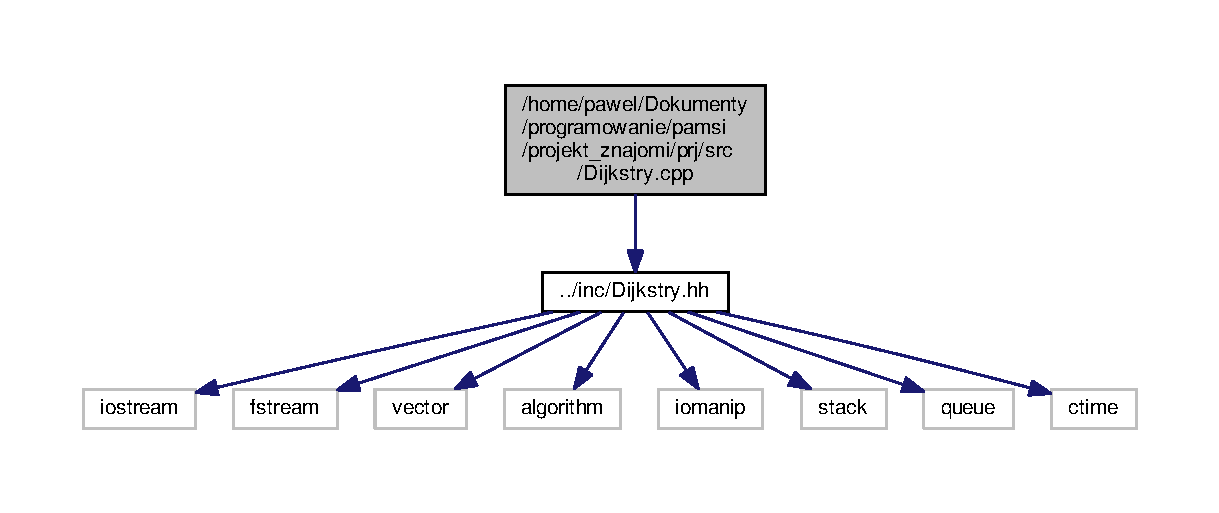
\includegraphics[width=350pt]{_dijkstry_8cpp__incl}
\end{center}
\end{figure}


\subsection{Detailed Description}
Plik zawiera funkcje z klasy graf. 

Definition in file \hyperlink{_dijkstry_8cpp_source}{Dijkstry.\-cpp}.

